




\documentclass{article}



\usepackage{amsmath}
\usepackage{amsfonts}
\usepackage{listings}

\usepackage[braket, qm]{qcircuit}
\usepackage{graphicx}





\title{Quantum Computing for Engineers}
\author{Osama Muhammad Raisuddin}







\begin{document}

\maketitle

\tableofcontents


  \vspace{10pt}
    \hrule
  \vspace{10pt}
This is the Abstract 
  \vspace{10pt}








\section{Introduction}


Quantum computing is an emerging area of research with great potential for engineering and scientific computing applications. Endowed with quantum mechanical properties such as superposition, entanglement and tunneling, quantum computers can enable exponential speedups over classical computers for some problems. The advantage can be realized in both time and energy consumption. 

All classical computation can be performed on quantum computers using reversible versions of logic gates. However, this approach is inefficient and required large overheads. To take advantage of quantum computers new algorithms have been developed and are an active area of research. Due to stark differences with classical computation, the engineering community has limited exposure to quantum computing and quantum algorithms. 

In this review we aim to provide an introduction to quantum computing with demonstration of concepts and ideas with code. Quantum algorithms relevant to engineers are presented in detail with implementation.




\section{Quantum Information}

\subsection{Quantum States}

\subsection{Operators}

\subsection{Measurements}

\subsection{Composite Systems}

\subsection{Density Operators}

\subsection{Born Rule}









This section should give an introduction to the state spaces of the qubits, operators, the Kronecker products, and densoty operator representation. 

The Born Rule needs to be introduced. The no-cloning theorem can also be introduced here.



\subsection{Postulates of Quantum Mechanics}

\subsubsection{State Space}

\subsubsection{Evolution}

\subsubsection{Measurement}

\subsubsection{Composite Systems}




\section{Quantum Computation}

In this section we abstract away details of quantum information and the underlying physics of a quantum computer and present the computational model for quantum computing. Since all gate-based quantum computers share the same computational model, this is a safe starting point for beginners. Implementation of quantum algorithms does not require knowledge beyond these fundamental elements.

\subsection{Qubits and Qudits}

A 'qubit', or a quantum bit, is the quantum analogue of a classical bit. It is the elementary information unit in quantum computing. A qubit is a two-dimensional quantum system with dimensions typically labelled '0' and'1' analogous to the states of a classical bit. A qubit is exists in the Hilbert space $ \mathcal{H} : \mathbb{C}^2$ and is represented in bra-ket (or Dirac) notation as:
\begin{equation}
\lvert \psi \rangle = \alpha \lvert 0 \rangle + \beta \lvert 1 \rangle
\end{equation}
where 
$ \lvert \alpha \rvert ^2 + \lvert \beta \rvert ^2 = 1$
 according to the Born rule and 
$ \lvert \psi \rangle \in \mathbb{C}^2$
 denotes the quantum state of the qubit. 
$ \lvert 0 \rangle$ and $ \lvert 1 \rangle $
 are the basis states in the 
$ 0-1$
 basis, corresponding to the basis vectors 
$ \lvert 0 \rangle = \begin{pmatrix}1 \\ 0\end{pmatrix} $
 and 
$ \lvert 1 \rangle = \begin{pmatrix}0 \\ 1\end{pmatrix} $
. 
$ \alpha $ and $ \beta $
 are the 'probability amplitudes' of the state 
$ \lvert \psi \rangle $
, corresponding to a probabilities of measuring the qubit $ \lvert \psi \rangle $ in states $ \lvert 0 \rangle $ and $ \lvert 1 \rangle $ with probailitities $ \lvert \alpha \rvert ^2 $ and $ \lvert \beta \rvert ^2 $ respectively. Note that once a measurement is performed on qubit $ \lvert \psi \rangle $ to obtain a measured state of either $ \lvert 0 \rangle $ or $ \lvert 1 \rangle $, the state $ \lvert \psi \rangle $ is destroyed and further measurements (without any other subsequent operations) will repeatedly yield the same state that was measured.

The state $ \lvert \psi \rangle $ is a 'ket'. The corresponding 'bra'  $\langle \psi \rvert$ is the adjoint, or the complex transpose of the 'ket'. As an example, the basis states form the kets
 $ \langle 0 \rvert =  \begin{pmatrix}
1 \; 0
\end{pmatrix} $
 and 
$\langle 1 \rvert =  \begin{pmatrix}
0 \; 1
\end{pmatrix} $.

A qudit is higher-dimensional generalization of of a qubit, s.t. $ \lvert \psi \rangle \in \mathbb{C}^d , \, d>2$.



\subsection{Registers of Qubits}

A register of qubits is a collection of $ n $ qubits, whose combined state is represented as the quantum system $ \lvert \psi \rangle \in  \mathbb{C}^{2^{n}}$, corresponding to a tensor product of the individual Hilbert spaces of the qubits.  The combined state $ \lvert \psi  \rangle $ of two individual qubits $ \lvert \psi _ 0 \rangle = \alpha_1 \lvert 0 \rangle + \beta_1 \lvert 1 \rangle $ and $ \lvert \psi _ 1 \rangle = \alpha_2 \lvert 0 \rangle + \beta_2 \lvert 1 \rangle $ may be represented in Dirac notation as a Kronecker product of the individual qubits with various equivalent notations:

\begin{multline}
\lvert \psi \rangle = \lvert \psi _ 1 \rangle \otimes \lvert \psi _ 2 \rangle 
= \lvert \psi _ 1 \rangle \lvert \psi _ 2 \rangle
= \lvert \psi _ 1 \psi _ 2 \rangle
\\
= (\alpha_1 \lvert 0 \rangle      + \beta_1 \lvert 1 \rangle)(\alpha_2 \lvert 0 \rangle      + \beta_2 \lvert 1 \rangle)
\\
= \alpha_1 \alpha_2 \lvert 0 \rangle \lvert 0 \rangle         
+ \alpha_1 \beta_2 \lvert 0 \rangle \lvert 1 \rangle      
+ \alpha_2 \beta_1 \lvert 1 \rangle\lvert 0 \rangle        
+ \beta_1 \beta_2 \lvert 1 \rangle\lvert 1 \rangle
\\
= \alpha_1 \alpha_2 \lvert 0 \rangle \otimes \lvert 0 \rangle         
+ \alpha_1 \beta_2 \lvert 0 \rangle  \otimes \lvert 1 \rangle      
+ \alpha_2 \beta_1 \lvert 1 \rangle  \otimes \lvert 0 \rangle        
+ \beta_1 \beta_2 \lvert 1 \rangle  \otimes \lvert 1 \rangle
\\
= \alpha_1 \alpha_2 \lvert 0  0 \rangle 
+ \alpha_1 \beta_2 \lvert 0 1 \rangle 
+ \alpha_2 \beta_1 \lvert 1  0 \rangle 
+ \beta_1 \beta_2 \lvert 1 1 \rangle
\\
= \alpha_1 \alpha_2        \begin{pmatrix}1\\0\end{pmatrix} \otimes \begin{pmatrix}1\\0\end{pmatrix} 
+ \alpha_2 \beta_1           \begin{pmatrix}1\\0\end{pmatrix} \otimes \begin{pmatrix}0\\1\end{pmatrix} 
+ \alpha_1 \beta_2            \begin{pmatrix}0\\1\end{pmatrix} \otimes \begin{pmatrix}1\\0\end{pmatrix} 
+ \beta_1 \beta_2               \begin{pmatrix}0\\1\end{pmatrix} \otimes \begin{pmatrix}0\\1\end{pmatrix} 
\\
= \alpha_1 \alpha_2        \begin{pmatrix}1\\0\\0\\0\end{pmatrix} 
+ \alpha_2 \beta_1           \begin{pmatrix}0\\1\\0\\0\end{pmatrix} 
+ \alpha_1 \beta_2            \begin{pmatrix}0\\0\\1\\0\end{pmatrix} 
+ \beta_1 \beta_2               \begin{pmatrix}0\\0\\0\\1\end{pmatrix} 
= \begin{pmatrix} \alpha_1 \alpha_2 \\  \alpha_2 \beta_1  \\  \alpha_1 \beta_2 \\  \beta_1 \beta_2 \end{pmatrix} 
 .
\end{multline}


Additonal qubits will follow the same pattern, resulting in an exponentially large state space for the qubits. Note that the ordering of qubits is arbitrary, and a change in ordering shuffles the representation of the state corresponding the Kronecker product; typically one may choose the most conventient order for their application.

%Here, we provide an example code in Qiskit to allocate a register of qubits:

%\lstinputlisting[language=Python]{code_snippets/qubit_register.py}






\subsection{Gates}

In the gate-based quantum computing model operations on qubits are represented as quantum gates, or simply gates. Some of the gates are analogous to classical gate operations. However, some quantum gates may not have a corresponding classical counterpart.

Gates can be conveniently represented as complex matrices, in line with the column vector representation of qubits. The most basic gates are single qubit gates represented as $\mathbb{C}^{2\times2}$. Some important single-qubit gates are  the Pauli gate set $\{I,X,Y,Z\}$ and the Hadamard gate $H$.

Gate can also act on multiple qubits, in which case they can be represented in $\mathbb{C}^{2^{n}\times2^{n}}$. Multiple qubit gates typically arise as controlled versions of gates, of which $CNOT$ is a commonly used one. The $SWAP$ gate is another common gate which swaps the states between qubits.

All quantum gates are unitary operations, which ensures normalization of quantum states in line with the Born rule. Consequantly, all quantum gates are also reversible operations, with the reverse operation simply being the Hermitian transpoise or conjugate transpose of the quantum gate.

Gates acting on qubits are typically represented as left multiplication. As an example, consider a register of three qubits in the state $ \lvert 000 \rangle $. Applying a Hadamard gate to the first qubit and a Pauli X gate to the last qubit (from the left) is represented as:

\begin{equation}
(H\otimes I\otimes X) \lvert 000 \rangle = (H \otimes I \otimes I) \lvert 001 \rangle = \frac{1}{\sqrt{2}} (\lvert 001 \rangle + \lvert 101 \rangle)
\end{equation}

As another example, consider a  register of two qubits with a Hadamard gate applied to the first qubit and a CNOT gate applied to the second qubit, controlled by the first qubit:

\begin{equation}
( \lvert 00 \rangle \langle 00 \rvert + 
\lvert 01 \rangle \langle 01 \rvert + 
\lvert 10 \rangle \langle 11 \rvert + 
\lvert 11 \rangle \langle 10 \rvert
 )(H \otimes I) \lvert 00 \rangle 
=
\lvert 00 \rangle + \lvert 11 \rangle 
\end{equation}

Note how the order of operations progresses from right to left. It is common practice not to include the $I$ gate when the qubits on which the operation is applied is implied.

Similar to classical Boolean logic, quantum gates can also form a universal gate set. This implies that any arbitrary quantum gate can be approximated using a universal gate set. The Solovay-Kitaev theorem is a central theorem in quantum computing which shows that the approximation error using a universal gate set scales as $ O (\log^c (\frac{1}{\epsilon}))$ for a single-qubit gate where $ c \approx 2$ and $O(m \log ^c (\frac{m}{\epsilon}))$ for a a set of $m$ $CNOT$s  and single-qubit unitaries. These correspond to a polylogarithmic increase in the original number of gates.

Underlying hardware implementations can have a variety of gate sets. Algorithms are typically agnostic to the hardware implementation, since the gates are converted to the target hardware's gate set in a process called transpilation.



\subsection{Measurement}

A quantum state is defined using probability amplitudes. In order to read a state a series of measurements of the state need to be performed, and the measurement statistics will correspond to the probability amplitudes of the quantum state.

In gate-based quantum computing projective measurements are typically used and are represented by a 'meter' symbol. The measurement operation is a projection onto the $ \lvert 0 \rangle $ $ \lvert 1 \rangle $ basis. As an example, consider a two-qubit system in the state $ \frac{1}{2} ( \lvert 00 \rangle + \lvert 01 \rangle + \lvert 10 \rangle + \lvert 11 \rangle )$, with a measurement being performed on the first qubit. If the first qubit is measured in the state $ \lvert 0 \rangle  $ , the final state is:
 \begin{equation}
( \rvert 0 \rangle \langle 0 \rvert \otimes I ) (\frac{1}{2} ( \lvert 00 \rangle + \lvert 01 \rangle + \lvert 10 \rangle + \lvert 11 \rangle ) )
=
\frac{1}{\sqrt{2}} (\lvert 00 \rangle + \lvert 01 \rangle )
\end{equation}

Similarly, if the first qubit is measured in the state $ \lvert 1 \rangle $ the final state is:

 \begin{equation}
( \rvert 1 \rangle \langle 1 \rvert \otimes I ) (\frac{1}{2} ( \lvert 00 \rangle + \lvert 01 \rangle + \lvert 10 \rangle + \lvert 11 \rangle ) )
=
\frac{1}{\sqrt{2}} (\lvert 10 \rangle + \lvert 11 \rangle )
\end{equation}


Measurements may be performed to either read out an entire quantum register or as a flag to indicate successful operation by measuring ancilla qubits.

Note that measurements will provide the squared moduli (amplitudes) of the complex numbers defining the probability amplitude of a quantum state. In order to recover additonal information, like the arguments (phases),  a process known as quantum state tomography [ref] is performed. Quantum states also have an overall phase. The overall phase is not measurable; only relative phase between two states is measurable.


%\subsubsection{Principle of Deferred Measurement}
%
%Measurement operations can usually be pushed forward till the end 

\subsection{Circuits}

Working with algebraic forms of algorithms can be unwieldy and difficult to visualize. Quantum circuits are a convenient representation of qubits and the operation sequence.





 As an example, consider a register of three qubits $\lvert A B C \rangle $, with an $H$ gate applied to the $A$ and an $X$ gate applied to $C$, followed by a $CNOT$ gate controlled by the $A$ applied to $B$, and finally measurements on all the qubits. These operations can conveniently be represented in circuit form as:



\begin{figure}[h]
\centering
\scalebox{1.0}{
\Qcircuit @C=1.0em @R=0.2em @!R { \\
	 	\nghost{A :  } & \lstick{A :  } & \gate{\mathrm{H}} & \ctrl{1} \barrier[0em]{2} & \qw & \meter & \qw & \qw & \qw & \qw\\
	 	\nghost{B :  } & \lstick{B :  } & \qw & \targ & \qw & \qw & \meter & \qw & \qw & \qw\\
	 	\nghost{C :  } & \lstick{C :  } & \gate{\mathrm{X}} & \qw & \qw & \qw & \qw & \meter & \qw & \qw\\
	 	\nghost{\mathrm{{Classical\;Bits} :  }} & \lstick{\mathrm{{Classical\;Bits} :  }} & \lstick{/_{_{3}}} \cw & \cw & \cw & \dstick{_{_{\hspace{0.0em}0}}} \cw \ar @{<=} [-3,0] & \dstick{_{_{\hspace{0.0em}1}}} \cw \ar @{<=} [-2,0] & \dstick{_{_{\hspace{0.0em}2}}} \cw \ar @{<=} [-1,0] & \cw & \cw\\
\\ }}

\caption{Circuit with gates and measurements.}
\label{fig:first_circuit}

\end{figure}


Note that the operations are ordered from left to right, unlike operations ordered right to left in algebraic notation. A controlled operation can be applied conditioned on the control qubit being either in the state $1$ or  $0$. This in indicated in a quantum circuit with a filled or empty circle respectively, as shown in Figure \ref{fig:gate_conditions}.

\begin{figure}[h]

\centering
\scalebox{1.0}{
\Qcircuit @C=1.0em @R=0.2em @!R { \\
	 	\nghost{A :  } & \lstick{A :  } & \ctrl{1} & \ctrlo{1} & \qw & \qw\\
	 	\nghost{B :  } & \lstick{B :  } & \targ & \targ & \qw & \qw\\
\\ }}

\caption{$CNOT$ gates conditioned on $A$ in states $0$ and $1$.}
\label{fig:gate_conditions}

\end{figure}



Quantum registers can be ordered using either little-endian or big-endian notation. Little-endian ordering corresponds to the right-most qubit in algeraic notation indexed as $0$ and big-endian corresponds to the left-most qubit indexed as $0$. Qiskit uses little-endian ordering.

As an example, we repeat the example in Figure \ref{fig:first_circuit} but with $\lvert ABC \rangle$ being denoted as $\lvert \psi \rangle$. Consistent with Qiskit, in little-endian notation $\lvert A\rangle$, $\lvert B\rangle$, and $\lvert C\rangle$ correspond to $\lvert \psi _2 \rangle$, $\lvert \psi _1 \rangle$, and $\lvert \psi _0 \rangle$. We provide an example code: starting with big-endian notation and converting to little-endian at the end.


\lstinputlisting[language=Python]{code_snippets/endian.py}




\begin{figure}[h]


\scalebox{1.0}{
\Qcircuit @C=1.0em @R=0.2em @!R { \\
	 	\nghost{{\psi}_{0} :  } & \lstick{{\psi}_{0} :  } & \gate{\mathrm{X}} & \qw \barrier[0em]{2} & \qw & \qw & \qw & \meter & \qw & \qw\\
	 	\nghost{{\psi}_{1} :  } & \lstick{{\psi}_{1} :  } & \qw & \targ & \qw & \qw & \meter & \qw & \qw & \qw\\
	 	\nghost{{\psi}_{2} :  } & \lstick{{\psi}_{2} :  } & \gate{\mathrm{H}} & \ctrl{-1} & \qw & \meter & \qw & \qw & \qw & \qw\\
	 	\nghost{\mathrm{{Classical\;Bits} :  }} & \lstick{\mathrm{{Classical\;Bits} :  }} & \lstick{/_{_{3}}} \cw & \cw & \cw & \dstick{_{_{\hspace{0.0em}0}}} \cw \ar @{<=} [-1,0] & \dstick{_{_{\hspace{0.0em}1}}} \cw \ar @{<=} [-2,0] & \dstick{_{_{\hspace{0.0em}2}}} \cw \ar @{<=} [-3,0] & \cw & \cw\\
\\ }}

\caption{Output of Example code}


\end{figure}




\subsection{Superposition}

Superposition is a central property of quantum computing. A quantum state can exist in a superposition of states. As an example, a single qubit $\lvert \psi \rangle$ can exist in a superposition of $\lvert 0 \rangle$ and $\lvert 1 \rangle$. A register of $n$ qubits can exist in an exponentially large superposition of $N=2^n$ states. The Hadamard gate puts qubits in superposition. As an example, we provide the following code to put qubits in uniform superposition and measure their states:

\begin{figure}[h]

\centering

\scalebox{1.0}{
\Qcircuit @C=1.0em @R=0.2em @!R { \\
	 	\nghost{{\psi}_{0} :  } & \lstick{{\psi}_{0} :  } & \gate{\mathrm{H}} & \meter & \qw & \qw & \qw & \qw\\
	 	\nghost{{\psi}_{1} :  } & \lstick{{\psi}_{1} :  } & \gate{\mathrm{H}} & \qw & \meter & \qw & \qw & \qw\\
	 	\nghost{{\psi}_{2} :  } & \lstick{{\psi}_{2} :  } & \gate{\mathrm{H}} & \qw & \qw & \meter & \qw & \qw\\
	 	\nghost{\mathrm{{Classical\;Bits} :  }} & \lstick{\mathrm{{Classical\;Bits} :  }} & \lstick{/_{_{3}}} \cw & \dstick{_{_{\hspace{0.0em}0}}} \cw \ar @{<=} [-3,0] & \dstick{_{_{\hspace{0.0em}1}}} \cw \ar @{<=} [-2,0] & \dstick{_{_{\hspace{0.0em}2}}} \cw \ar @{<=} [-1,0] & \cw & \cw\\
\\ }}

\caption{Circuit for uniform superposition.}

\end{figure}


\lstinputlisting[language=Python]{code_snippets/uniform_superposition.py}

\begin{figure}[h]
\centering

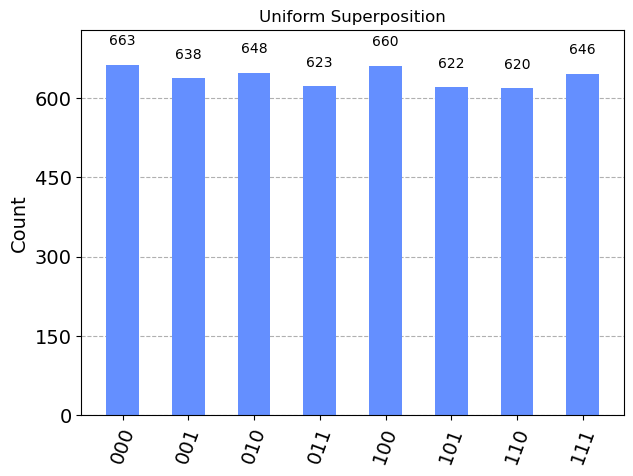
\includegraphics[scale=0.5]{code_snippets/uniform_superposition_output.png}


\caption{Output of Uniform Superposition code}

\end{figure}



\subsection{Entanglement}

Entanglement is another property unique to quantum computation. Entangled qubits have a correlated state. 

Note that entangled qubits cannot be seperated into a Kronecker product, at least not without an auxiliary variable.

\subsection{Reversible Computation}



This is the most detailed section. Over here we abstract away all the details about physics etc. and will only work with qubits and circuits.

We will introduce single and multiple qubits, and gate for single and multiple qubits. Controlled gates will also be introduced.

Then we talk about measurements. We will use projective measurements in the standard basis.

The ideas of superposition, entanglement, (and interference?) will be introduced. We will also mention that all operations are reversible, and reversible versions of classical operations can be done in reversible circuits, but this has lage overheads.

Talk about data representation, amplitude encoding is the important one.

Talk about the big limitations.

Inroduce some 

\section{Quantum Algorithms for Engineering}








\end{document}

